% Soubory musí být v kódování, které je nastaveno v příkazu \usepackage[...]{inputenc}

\documentclass[%        Základní nastavení
  %draft,    				  % Testovací překlad
  12pt,       				% Velikost základního písma je 12 bodů
	t,                  % obsah slajdů bude vždy začínat od shora (nebude vertikálně centrovaný)
	aspectratio=1610,   % poměr stran bude 16:10 (všechny projektory v učebnách na Technické 12 Brno),
	                    % další volby jsou 43, 149, 169, 54, 32.
	unicode,						% Záložky a informace budou v kódování unicode
]{beamer}				    	% Dokument třídy 'zpráva', vhodná pro sazbu závěrečných prací s kapitolami
%\usepackage{etex}

\usepackage[utf8]		  % Kódování zdrojových souborů je v UTF-8
	{inputenc}					% Balíček pro nastavení kódování zdrojových souborů
	
\usepackage{graphicx} % Balíček 'graphicx' pro vkládání obrázků
											% Nutné pro vložení logotypů školy a fakulty

\usepackage[          % Balíček 'acronym' pro sazby zkratek a symbolů
	nohyperlinks				% Nebudou tvořeny hypertextové odkazy do seznamu zkratek
]{acronym}						
											% Nutné pro použití prostředí 'acronym' balíčku 'thesis'

%% Balíček hyperref je volán třídou beamer automaticky, proto není třeba následujícího kódu:
%\usepackage[
%	breaklinks=true,		% Hypertextové odkazy mohou obsahovat zalomení řádku
%	hypertexnames=false % Názvy hypertextových odkazů budou tvořeny
%											% nezávisle na názvech TeXu
%]{hyperref}						% Balíček 'hyperref' pro sazbu hypertextových odkazů
%											% Nutné pro použití příkazu 'nastavenipdf' balíčku 'thesis'

\usepackage{cmap} 		% Balíček cmap zajišťuje, že PDF vytvořené `pdflatexem' je
											% plně "prohledávatelné" a "kopírovatelné"

%\usepackage{upgreek}	% Balíček pro sazbu stojatých řeckých písmem
											%% např. stojaté pí: \uppi
											%% např. stojaté mí: \upmu (použitelné třeba v mikrometrech)
											%% pozor, grafická nekompatibilita s fonty typu Computer Modern!

%\usepackage{amsmath} %balíček pro sabu náročnější matematiky

\usepackage{booktabs} % Balíček, který umožňuje v tabulce používat
                      % příkazy \toprule, \midrule, \bottomrule


%%%%%%%%%%%%%%%%%%%%%%%%%%%%%%%%%%%%%%%%%%%%%%%%%%%%%%%%%%%%%%%%%
%%%%%%      Definice informací o dokumentu             %%%%%%%%%%
%%%%%%%%%%%%%%%%%%%%%%%%%%%%%%%%%%%%%%%%%%%%%%%%%%%%%%%%%%%%%%%%%

% V tomto souboru se nastavují téměř veškeré informace, proměnné mezi studenty:
% jméno, název práce, pohlaví atd.
% Tento soubor je SDÍLENÝ mezi textem práce a prezentací k obhajobě -- netřeba něco nastavovat na dvou místech.

\usepackage[
%%% Z následujících voleb jazyka lze použít pouze jednu
  %czech-english,		% originální jazyk je čeština, překlad je anglicky (výchozí)
  %english-czech,	% originální jazyk je angličtina, překlad je česky
  slovak-english,	% originální jazyk je slovenština, překlad je anglicky
  %english-slovak,	% originální jazyk je angličtina, překlad je slovensky
%
%%% Z následujících voleb typu práce lze použít pouze jednu
  semestral,		  % semestrální práce (nesází se abstrakty, prohlášení, poděkování) (výchozí)
  %bachelor,			%	bakalářská práce
  %master,			  % diplomová práce
  %treatise,			% pojednání o disertační práci
  %doctoral,			% disertační práce
%
%%% Z následujících voleb zarovnání objektů lze použít pouze jednu
%  left,				  % rovnice a popisky plovoucích objektů budou zarovnány vlevo
	center,			    % rovnice a popisky plovoucích objektů budou zarovnány na střed (vychozi)
%
]{thesis}   % Balíček pro sazbu studentských prací

% jediný autor: šablona pre semestrálny projekt predpokladá viacerých
\makeatletter
\renewcommand\autortext@slovak{Autor projektu}
\renewcommand\autortext@english{Author}
\makeatother


%%% Jméno a příjmení autora ve tvaru
%  [tituly před jménem]{Křestní}{Příjmení}[tituly za jménem]
% Pokud osoba nemá titul před/za jménem, smažte celý řetězec '[...]'
\author{Martin}{Szuc}

%%% Identifikační číslo autora (VUT ID)
\butid{231284}

%%% Pohlaví autora/autorky
% (nepoužije se ve variantě english-czech ani english-slovak)
% Číselná hodnota: 1...žena, 0...muž
\gender{0}

%%% Jméno a příjmení vedoucího/školitele včetně titulů
%  [tituly před jménem]{Křestní}{Příjmení}[tituly za jménem]
% Pokud osoba nemá titul před/za jménem, smažte celý řetězec '[...]'
\advisor[Ing.]{David}{Zeman}

%%% Jméno a příjmení oponenta včetně titulů
%  [tituly před jménem]{Křestní}{Příjmení}[tituly za jménem]
% Pokud osoba nemá titul před/za jménem, smažte celý řetězec '[...]'
% Nastavení oponenta se uplatní pouze v prezentaci k obhajobě;
% v případě, že nechcete, aby se na titulním snímku prezentace zobrazoval oponent, pouze příkaz zakomentujte;
% u obhajoby semestrální práce se oponent nezobrazuje (jelikož neexistuje)
% U dizertační práce jsou typicky dva až tři oponenti. Pokud je chcete mít na titulním slajdu, prosím ručně odkomentujte a upravte jejich jména v definici "VUT title page" v souboru thesis.sty.
%\opponent[doc.\ Mgr.]{Křestní}{Příjmení}[Ph.D.]

%%% Název práce
%  Parametr ve složených závorkách {} je název v originálním jazyce,
%  parametr v hranatých závorkách [] je překlad (podle toho jaký je originální jazyk).
%  V případě, že název Vaší práce je dlouhý a nevleze se celý do zápatí prezentace, použijte příkaz
%  \def\insertshorttitle{Zkác.\ náz.\ práce}
%  kde jako parametr vyplníte zkrácený název. Pokud nechcete zkracovat název, budete muset předefinovat,
%  jak se vytváří patička slidu. Viz odkaz: https://bit.ly/3EJTp5A
\title[Zero-trust access and access control in a container environment]{Zero-trust prístup a riadenie prístupu v containerovom prostredí}

%%% Označení oboru studia
%  Parametr ve složených závorkách {} je název oboru v originálním jazyce,
%  parametr v hranatých závorkách [] je překlad
\specialization[Information Security]{Informačná bezpečnosť}

%%% Označení ústavu
%  Parametr ve složených závorkách {} je název ústavu v originálním jazyce,
%  parametr v hranatých závorkách [] je překlad
%\department[Department of Control and Instrumentation]{Ústav automatizace a měřicí techniky}
%\department[Department of Biomedical Engineering]{Ústav biomedicínského inženýrství}
%\department[Department of Electrical Power Engineering]{Ústav elektroenergetiky}
%\department[Department of Electrical and Electronic Technology]{Ústav elektrotechnologie}
%\department[Department of Physics]{Ústav fyziky}
%\department[Department of Foreign Languages]{Ústav jazyků}
%\department[Department of Mathematics]{Ústav matematiky}
%\department[Department of Microelectronics]{Ústav mikroelektroniky}
%\department[Department of Radio Electronics]{Ústav radioelektroniky}
%\department[Department of Theoretical and Experimental Electrical Engineering]{Ústav teoretické a experimentální elektrotechniky}
\department[Department of Telecommunications]{Ústav telekomunikací}
%\department[Department of Power Electrical and Electronic Engineering]{Ústav výkonové elektrotechniky a elektroniky}

%%% Označení fakulty
%  Parametr ve složených závorkách {} je název fakulty v originálním jazyce,
%  parametr v hranatých závorkách [] je překlad
%\faculty[Faculty of Architecture]{Fakulta architektury}
\faculty[Faculty of Electrical Engineering and~Communication]{Fakulta elektrotechniky a~komunikačních technologií}
%\faculty[Faculty of Chemistry]{Fakulta chemická}
%\faculty[Faculty of Information Technology]{Fakulta informačních technologií}
%\faculty[Faculty of Business and Management]{Fakulta podnikatelská}
%\faculty[Faculty of Civil Engineering]{Fakulta stavební}
%\faculty[Faculty of Mechanical Engineering]{Fakulta strojního inženýrství}
%\faculty[Faculty of Fine Arts]{Fakulta výtvarných umění}
%
%Nastavení logotypu (v hranatych zavorkach zkracene logo, ve slozenych plne):
\facultylogo[logo/FEKT_zkratka_barevne_PANTONE_CZ]{logo/UTKO_color_PANTONE_CZ}

%%% Rok odevzdání práce
\graduateyear{2026}

%%% Datum obhajoby (uplatní se pouze v prezentaci k obhajobě)
\date{1.\,12.\,2026} 

%%% Místo obhajoby
% Na titulních stránkách bude automaticky vysázeno VELKÝMI písmeny (pokud tyto stránky sází šablona)
\city{Brno}
      % v tomto souboru doplňte údaje o sobě, o názvu práce...
                       % (tento soubor je sdílený s textem práce)

%%%%%%%%%%%%%%%%%%%%%%%%%%%%%%%%%%%%%%%%%%%%%%%%%%%%%%%%%%%%%%%%%%%%%%%%

%%%%%%%%%%%%%%%%%%%%%%%%%%%%%%%%%%%%%%%%%%%%%%%%%%%%%%%%%%%%%%%%%%%%%%%%
%%%%%%     Nastavení polí ve Vlastnostech dokumentu PDF      %%%%%%%%%%%
%%%%%%%%%%%%%%%%%%%%%%%%%%%%%%%%%%%%%%%%%%%%%%%%%%%%%%%%%%%%%%%%%%%%%%%%
%% Při vloženém balíčku 'hyperref' lze použít příkaz '\pdfsettings'
\pdfsettings
%  Nastavení polí je možné provést také ručně příkazem:
%\hypersetup{
%  pdftitle={Název studentské práce},    	% Pole 'Document Title'
%  pdfauthor={Autor studenstké práce},   	% Pole 'Author'
%  pdfsubject={Typ práce}, 						  	% Pole 'Subject'
%  pdfkeywords={Klíčová slova}           	% Pole 'Keywords'
%}
\hypersetup{pdfpagemode=FullScreen}       % otevření rovnou v režimu celé obrazovky
%%%%%%%%%%%%%%%%%%%%%%%%%%%%%%%%%%%%%%%%%%%%%%%%%%%%%%%%%%%%%%%%%%%%%%%

\usetheme{VUT} 				% barvy a rozložení prezentace odpovídající VUT FEKT
% alternativně lze použít jiná berevná témata, ale bez záruky. Například: 
%\usetheme{Darmstadt} \usecolortheme{default2}
\logoheader					% vytvoření zkráceného loga VUT FEKT v hlavičce slajdu, nechte odkomentované



\begin{document}

% v případě zakomentování následujícího se zobrazí v pravém dolním rohu slajdů klikatelné navigační symboly 
\disablenavigationsymbols

% titulní snímek, vysazen bez horních, dolních a postranních lišt (volba plain),
% není tak vysazen ani nadpis snímku
\maketitle

%%%%%%%%%%%%%%%%%%%%%%%%%%%%%%%%%%%%%%%%%%%%%%%%%%%%%%%%%%%%%%%%%%%%%%%

\begin{frame}
  \frametitle{Zadanie a otázka}
  \begin{itemize}
    \item Analýza prístupov k segmentácii siete a autentizácii v mikroslužbách
    \item Konfigurácia a testovanie bezpečného prepojenia izolovaných uzlov
    \item Meranie réžie
  \end{itemize}
  \vspace{1em}
  \textbf{Otázka:} pred čím chráni ktorá vrstva zero trust v Kubernetes a koľko stojí?
  \vspace{1em}
  \begin{itemize}
    \item kontrolovaný experiment: každá konfigurácia pridá práve jeden prvok
    \item každý test zodpovedá hrozbe, každé meranie jednému prvku
  \end{itemize}
\end{frame}

\begin{frame}
  \frametitle{Model hrozieb}
  Útočník spúšťa kód v jednom pode alebo počúva na sieti medzi uzlami.
  \vspace{0.5em}
  \small
  \begin{tabular}{@{}ll@{}}
    \toprule
    Útok & Cieľ \\
    \midrule
    Laterálny pohyb & frontend číta databázu priamo \\
    Odpočúvanie siete & obsah a metadáta prevádzky medzi uzlami \\
    Podvrhnutie identity & pod s cudzím labelom alebo ServiceAccountom \\
    Neoprávnená operácia & zápis tam, kde je povolené iba čítanie \\
    Kompromitovaná služba & platná identita aj povolená cesta \\
    Zneužitie tokenu & ServiceAccount token proti API serveru \\
    \bottomrule
  \end{tabular}
\end{frame}

\begin{frame}
  \frametitle{Testovacie prostredie}
  \centering
  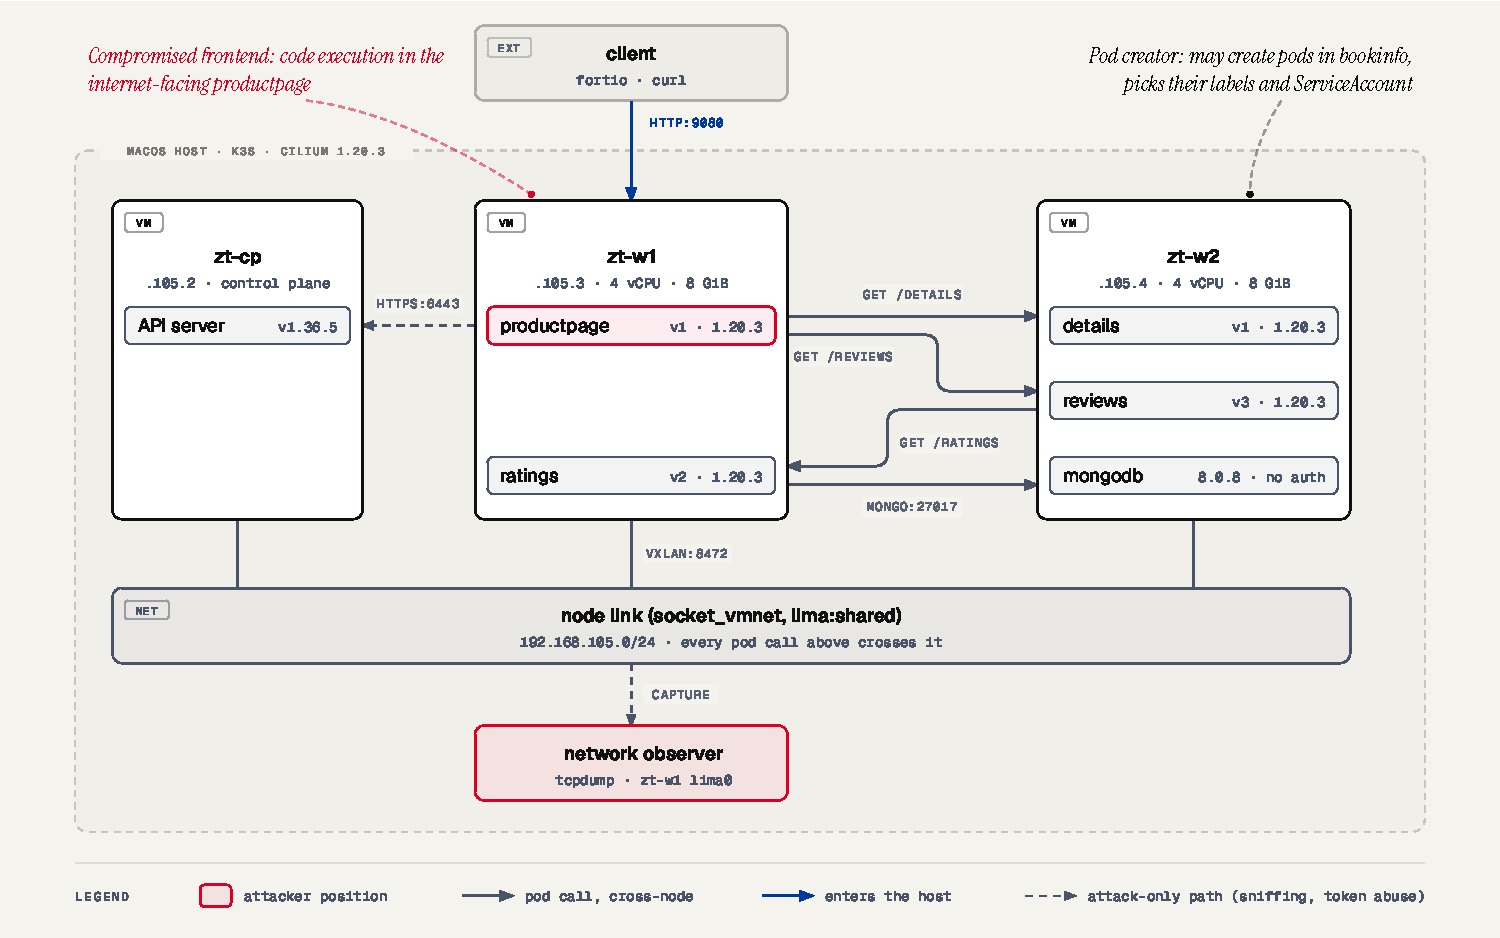
\includegraphics[width=\textwidth,height=0.72\textheight,keepaspectratio]{../figures/testbed.pdf}
  \par\small 3 virtual machines (Lima, arm64), k3s, Cilium 1.20, Istio 1.30, Bookinfo
\end{frame}

\begin{frame}
  \frametitle{Konfigurácie}
  \centering
  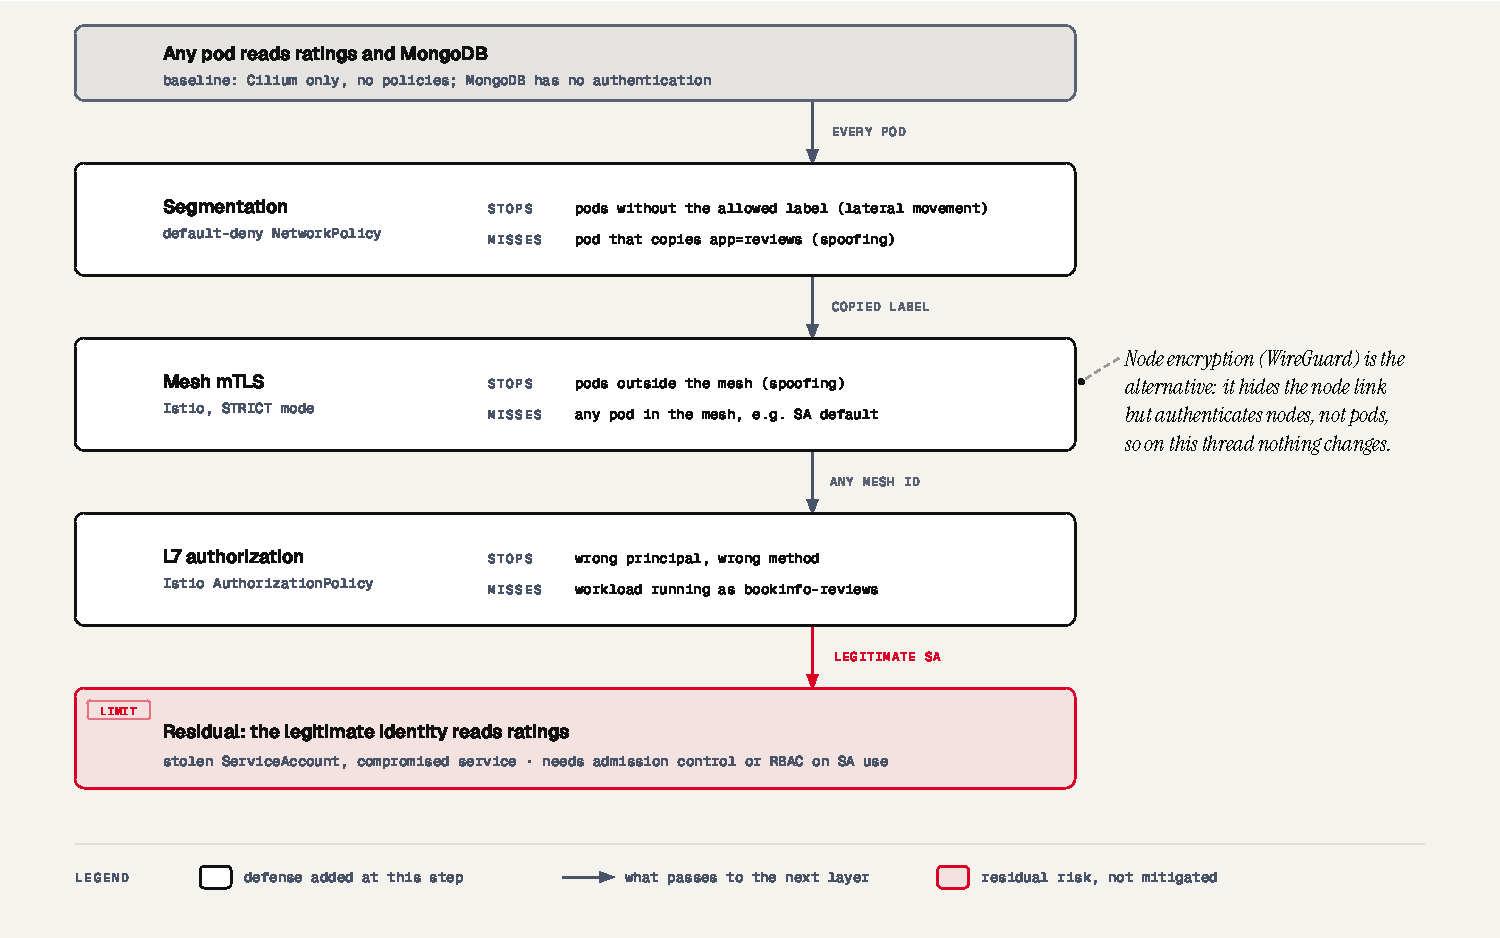
\includegraphics[width=\textwidth,height=0.78\textheight,keepaspectratio]{../figures/scenario-layers.pdf}
\end{frame}

\begin{frame}
  \frametitle{Výsledky útokov}
  \scriptsize
  \setlength{\tabcolsep}{4pt}
  \begin{tabular}{@{}lccccc@{}}
    \toprule
    Útok & Bez ochrany & Segmentácia & WireGuard & mTLS & L7 autorizácia \\
    \midrule
    Laterálny pohyb & prejde & \textbf{zastavený} & zastavený & zastavený & zastavený \\
    Odpočúvanie, obsah & prejde & prejde & \textbf{zastavený} & \textbf{zastavený} & zastavený \\
    Odpočúvanie, metadáta & prejde & prejde & \textbf{zastavený} & prejde & prejde \\
    Podvrhnutie, mimo mesh & prejde & prejde & prejde & \textbf{zastavený} & zastavený \\
    Podvrhnutie, iný SA & prejde & prejde & prejde & prejde & \textbf{zastavený} \\
    Podvrhnutie, ukradnutý SA & prejde & prejde & prejde & prejde & prejde \\
    Neoprávnená operácia & prejde & prejde & prejde & prejde & \textbf{zastavený} \\
    Kompromitovaná služba & prejde & prejde & prejde & prejde & prejde \\
    Zneužitie tokenu & prejde & \textbf{zastavený} & zastavený & zastavený & zastavený \\
    \bottomrule
  \end{tabular}
  \vspace{0.8em}
  \par\small 70 automatizovaných kontrol, všetky podľa hypotéz; \texttt{make test}
\end{frame}

\begin{frame}
  \frametitle{Ktorý prvok útok zastavil}
  \small
  \begin{tabular}{@{}lll@{}}
    \toprule
    Prvok & Útočník vidí & Dôkaz v clustri \\
    \midrule
    Segmentácia & \texttt{timed out} & Hubble: \texttt{Policy denied} \\
    mTLS & \texttt{Connection reset} & sidecar odmietne plaintext \\
    L7 autorizácia & HTTP 403 & \texttt{RBAC: access denied} \\
    \bottomrule
  \end{tabular}
  \vspace{1em}
  \begin{itemize}
    \item každé zastavenie sa dá priradiť práve jednému prvku
    \item ukážka: \texttt{make s1 \&\& make test}, potom \texttt{make s3 \&\& make test}
  \end{itemize}
\end{frame}

\begin{frame}
  \frametitle{WireGuard verzus mTLS}
  \small
  \begin{tabular}{@{}lcc@{}}
    \toprule
     & WireGuard medzi uzlami & mTLS medzi službami \\
    \midrule
    Šifruje obsah medzi uzlami & áno & áno \\
    Skryje adresy podov a porty & áno & nie \\
    Šifruje prevádzku na jednom uzle & nie & áno \\
    Autentizuje & uzly & workloady \\
    Zastaví pod mimo mesh & nie & áno \\
    \bottomrule
  \end{tabular}
  \vspace{1em}
  \begin{itemize}
    \item mTLS: z jedného záznamu sa dá zostaviť celý graf volaní
    \item pre bezpečné prepojenie uzlov stačí WireGuard; na identitu služby treba mTLS
  \end{itemize}
\end{frame}

\begin{frame}
  \frametitle{Réžia: latencia}
  \centering
  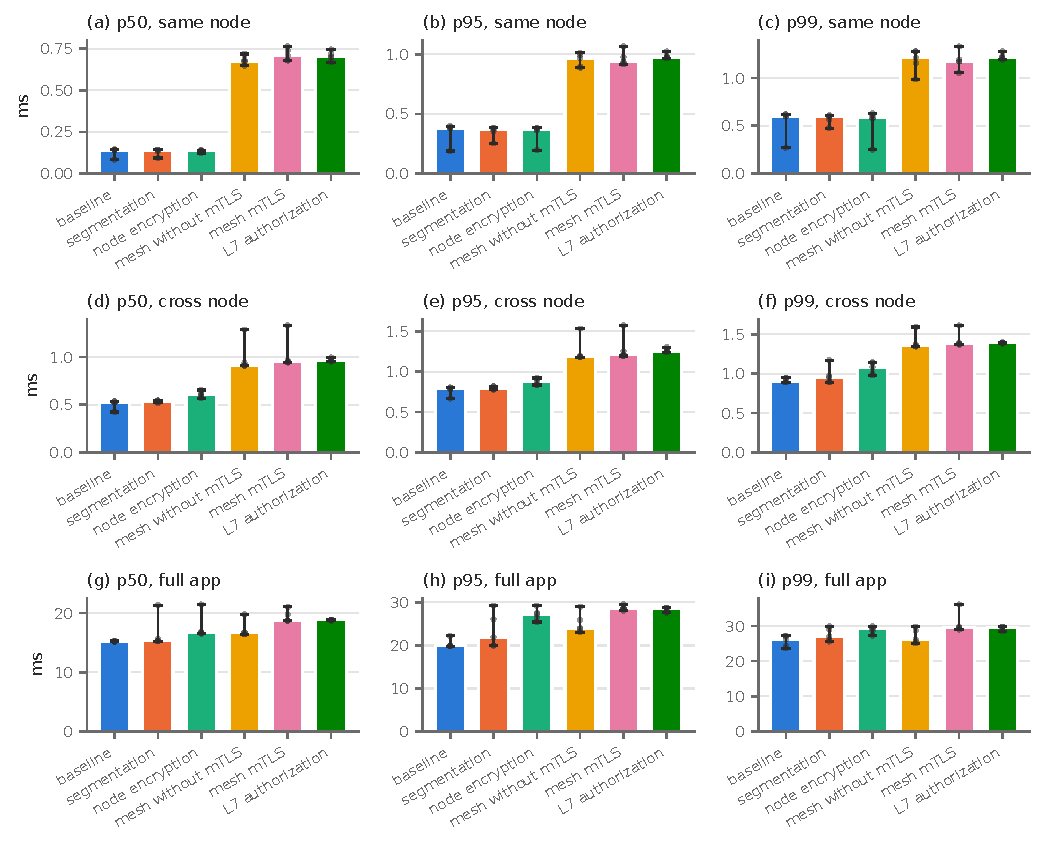
\includegraphics[width=\textwidth,height=0.75\textheight,keepaspectratio]{../figures/bench/latency.pdf}
\end{frame}

\begin{frame}
  \frametitle{Réžia: čo stojí ktorý prvok}
  \begin{itemize}
    \item \textbf{Segmentácia, L7 autorizácia:} do 1~\%
    \item \textbf{WireGuard:} medzi uzlami 2,7-krát viac CPU na Gbit/s
    \item \textbf{Sidecar:} väčšina ceny mesh, približne +0,5~ms na skok,\\ maximum záťaže medzi uzlami z 26\,500 na 10\,500 požiadaviek/s,\\ +200~MiB pamäte na uzol
    \item \textbf{mTLS v proxy:} na jednom uzle o 56~\% nižšia priepustnosť
  \end{itemize}
  \vspace{0.5em}
  \small Zistenie navyše: WireGuard zníži MTU všetkých trás podov, čo zrýchli aj prevádzku na jednom uzle (overené kontrolným meraním).
\end{frame}

\begin{frame}
  \frametitle{Obmedzenia}
  \begin{itemize}
    \item útočník s platnou identitou prejde všetkými vrstvami
    \item pod s ukradnutým ServiceAccountom: treba RBAC a admission control
    \item obídenie sidecaru, metadáta pri mTLS
    \item žiadna identita používateľa ani zariadenia
    \item 17 politík pre 5 služieb, každá zmena aplikácie mení 2 až 3 politiky
    \item merané na notebooku: platia iba relatívne rozdiely
  \end{itemize}
\end{frame}

\begin{frame}
  \frametitle{Záver}
  \begin{itemize}
    \item segmentácia: prvý krok, prakticky zadarmo, ale dôveruje labelom
    \item WireGuard: lacné šifrovanie uzlov, neautentizuje workloady
    \item mTLS: identita služby, cenu tvorí hlavne sidecar
    \item autentizácia nie je autorizácia: podvrhnutie zastaví až L7 politika
    \item všetko reprodukovateľné: \url{https://github.com/martinszuc/fekt-mpc-ct3-zerotrust-k8s}
  \end{itemize}
\end{frame}

\begin{frame}[c]
  \frametitle{\mbox{ }}
  \begin{center}
    {\Huge Ďakujem za pozornosť.}
  \end{center}
\end{frame}

\end{document}
